\section{Data Cleaning on GRR Views}
The first part of our solution to Problem 2 relates to modeling the data cleaning.
We describe how data cleaning affects the statistics of queries on a GRR view.
To do so, we will have to keep track of provenance, i.e.,  the mapping between original values before data cleaning and the values after cleaning.
Since the predicates of our queries apply to single discrete attributes, and our data cleaning is applied to the partitioned groups $g_i$, without loss of generality, we present this section for only a single partitioned group $g_i$.

\subsection{Value Provenance Graph}
The local cleaning model defines a directed bipartite graph over distinct values.
Let $L$ be the set of distinct values of the GRR view before data cleaning, and let $M$ be the set of distinct values after data cleaning. Each $l \in L$ and each $m \in M$ defines a node in the bipartite graph. 
We add edges between $L$ and $M$ to represent the transformation made by a local cleaner.
However, even with deterministic local cleaners, there might be a many-to-one mapping.
It turns out that the deterministic local cleaner definition disallows one-to-many mappings, and we will exploit this structure for query result estimation.
An example of a \emph{one-to-many} local cleaner is one that with probability $0.5$ assigns one value or assigns another; a model which while theoretically possible is uncommon.

\begin{lemma}
Let $g_i$ be an discrete attribute partition, and $C_i$ be a local cleaner. The directed bipartite graph generated from $V$ and $V_{clean}$ is \textbf{fork-free}, that is there are no one-to-many mappings.
\end{lemma}

\begin{figure}[t]
\centering
 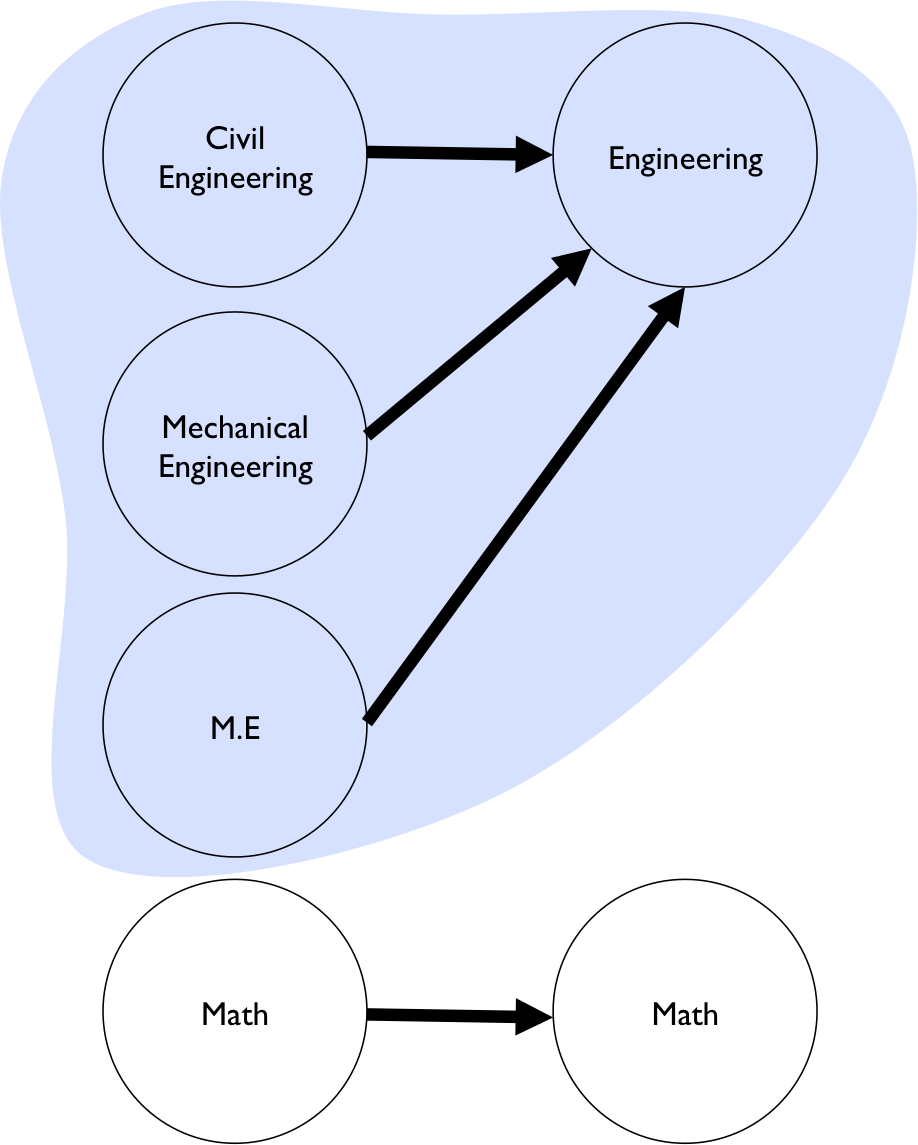
\includegraphics[width=0.5\columnwidth]{figs/graph.png}
 \caption{Local data cleaning operations can be described as a bipartite graph mapping old values to new ones. Predicates on cleaned relations can be interpreted as vertex cuts on the clean partition of the graph.\label{architecture}}
\end{figure}

\subsection{Predicates As Vertex Cuts}
Intuitively, the goal is for any predicate, which can be thought of as a subset of $M$, to quantify the false positive rate (records falsely included) and false negative rate (records falsely excluded) due to the randomization. 
This graph gives us a convenient abstraction to essentially count the number of edges affected by a predicate.
We consider predicates over a single attribute $d_i$.
Let $cond(d_i)$ be a predicate and each predicate can be expressed as a subset $M_{pred} \subseteq M$.
Each $L_{pred}$ will have a parent set $L_{pred}$, that is the set of vertices in $L$ with an edge to exactly one $m \in M_{pred}$.
Together $cut = (L_{pred},M_{pred})$ defines a cut on the bipartite graph.

\begin{example}
Suppose we have a dirty \textsf{major} of four values ``Civil Engineering", ``Mechanical Engineering", ``M.E", ``Math".
The local cleaner maps the first three values to ``Engineering", and the user's predicate queries ``Engineering".
$L_{pred}$ is the set that contains ``Civil Engineering", ``Mechanical Engineering", ``M.E".
$M_{pred}$ is singleton set with ``Engineering".
\end{example}

\begin{example}
Now let us consider an example with multiple attributes in $g_i$, and suppose $g_i$ was (\textsf{city}, \textsf{state}). 
The view has ``San Francisco, CA", ``San Francisco, NULL", ``New York, NY".
The local cleaner maps ``San Francisco, NULL" to ``San Francisco, CA", and if the user's predicate queries the \textsf{state} ``CA", then $L_{pred}$ is ``San Francisco, CA", ``San Francisco, NULL", and $M_{pred}$ is the singleton with ``San Francisco, CA".
\end{example}

\subsection{Predicate Probability Estimation}
When the user issues an aggregate query to a GRR view, there will be a false positive (records falsely included) and false negative rate (records falsely excluded).
Using this graph, we can estimate the false positive and false negative rates of a predicate.
Let $r \in R$ be a row from the original non-private relation.
Let $r' \in R_{clean}$ be a row from the hypothetical cleaned non-private relation.
Making the assumption from the section that the dataset is large enough such that the entire domain is visible in the GRR view and the fork-free nature of the bipartite graph, it is easy verify the following lemma:
\begin{lemma}\label{pre-image}
For an attribute $d_i \in g_i$, if and only if $cond(r'[d_i])$ is true then $r[d_i] \in L_{pred}$.
\end{lemma} 

Following from this lemma, to quantify the false positive and false negative rates of the predicate, we need to estimate the probability that after randomization a record is falsely in $L_{pred}$ or falsely excluded from $L_{pred}$ respectively.
Let $l = \mid L_{pred} \mid$, and $r[d_i] \in L_{pred}$.
The true positive probability is: 
\[
\tau_p = (1-p) + p \frac{l}{N}
\]
The false positive probability is: 
\[
\tau_n = p \frac{l}{N}
\]
Likewise, suppose $r[d_i] \not\in L_{pred}$, the true negative probability is:
\[
\gamma_p = (1-p) + p \frac{N-l}{N}
\]
and the false negative probability is:
\[
\gamma_n = p \frac{N-l}{N}
\]

From a statistical estimation perspective $p$ and $l$ are deterministic values known to the query processing system.
Therefore, $\tau_p,\tau_n,\gamma_p,\gamma_n$ are deterministic values.
In the following section, we show that this determinism allows for unbiased estimates of the aggregate queries.

\subsection{Note About Assumptions}
In proving Lemma \ref{pre-image}, we apply two assumptions: the dataset is large enough such that the entire domain is visible in the GRR view and the fork-free nature of the bipartite graph.
This lemma is instrumental in calculating deterministic values for $\tau_p,\tau_n,\gamma_p,\gamma_n$.
However, without these assumptions it is significantly harder to estimate $\tau_p,\tau_n,\gamma_p,\gamma_n$, since the lemma is no longer true.
If the entire domain is not visible in the private view, then the problem requires some sort of species estimation to estimate the number of missed values in $L_{pred}$ \cite{haas1995sampling}.
If the provenance graph is not fork-free then each of the edges will have to be weighted by the relative fraction of records transformed in certain way.
We would have to estimate this from the GRR view.
The result is that $\tau_p,\tau_n,\gamma_p,\gamma_n$ would be random variables and would have to be bounded in any analysis. 




